\subsection*{Pertanyaan: Analisis graf pada Gambar 9.2 dan tuliskan satu solusi jalur terpendek yang mungkin menggunakan algoritma A* apabila jarak heuristiknya merupakan banyaknya busur minimal dari node asal ke node target!}

\textbf{Graf Gambar 9.2:} Edge berbobot: 0--1 = 3, 0--2 = 4, 0--3 = 5, 1--3 = 2, 2--4 = 4, 3--4 = 2, 4--5 = 1, 4--6 = 5, dan 5--6 = 3. Start = 0, target = 6.

\begin{figure}[H]
    \centering
    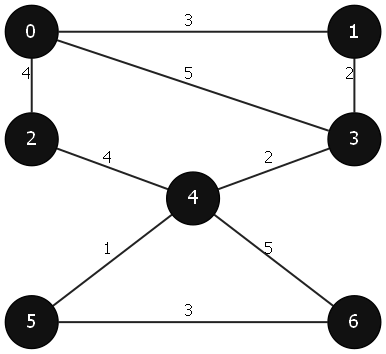
\includegraphics[width=0.52\textwidth]{figures/praktikum9/graf_pretest_92.png}
    \caption{Visualisasi Graf Pre Test dan Post Test Praktikum 9}
    \label{fig:praktikum9-graf-pretest}
\end{figure}

\textbf{Nilai heuristik:}
\begin{table}[H]
    \centering
    \caption{Nilai Heuristik Banyaknya Busur Minimum ke Node 6}
    \label{tab:praktikum9-heuristik}
    \begin{tabular}{cccccccc}
    \toprule
    \textbf{Node} & 0 & 1 & 2 & 3 & 4 & 5 & 6 \\ \midrule
    \textbf{$h(n)$} & 3 & 3 & 2 & 2 & 1 & 1 & 0 \\ \bottomrule
    \end{tabular}
\end{table}

\textbf{Penelusuran manual:}
\begin{table}[H]
    \centering
    \caption{Penelusuran Manual A* dari Node 0 ke Node 6}
    \label{tab:praktikum9-pretest-manual}
    \begin{tabularx}{\textwidth}{c l X X}
    \toprule
    \textbf{Langkah} & \textbf{Node} & \textbf{Kandidat Terbaik} & \textbf{Keterangan} \\ \midrule
    1 & 0 & 1: $f=6$, 2: $f=6$, 3: $f=7$ & Node 1 dan 2 terkecil. \\
    2 & 1 & 3: $f=7$ & Jalur ke 3 masih bernilai 7. \\
    3 & 2 & 4: $f=9$ & Jalur 0--2--4 menjadi kandidat. \\
    4 & 3 & 4: $f=8$ & Jalur ke 4 diperbaiki. \\
    5 & 4 & 5: $f=9$, 6: $f=12$ & Node 5 dipilih. \\
    6 & 5 & 6: $f=11$ & Jalur ke target diperbaiki. \\
    7 & 6 & selesai & Target tercapai. \\ \bottomrule
    \end{tabularx}
\end{table}

\textbf{Jawaban:}
\[
    0 \rightarrow 3 \rightarrow 4 \rightarrow 5 \rightarrow 6
\]
dengan total cost:
\[
    5 + 2 + 1 + 3 = 11
\]

\begin{figure}[H]
    \centering
    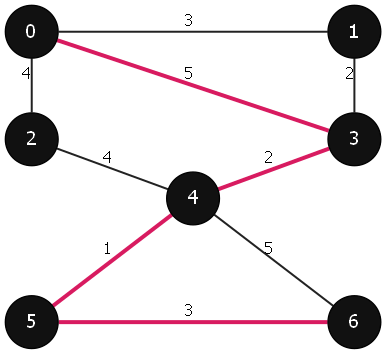
\includegraphics[width=0.52\textwidth]{figures/praktikum9/graf_pretest_92_solusi.png}
    \caption{Solusi Jalur Terpendek A* pada Graf Gambar 9.2}
    \label{fig:praktikum9-graf-pretest-solusi}
\end{figure}
